\documentclass[10.5pt,a4paper]{article}

\usepackage[margin=1.65cm]{geometry}
\usepackage[T1]{fontenc}
\usepackage{lmodern}
\usepackage{microtype}
\usepackage{amsmath,amssymb}
\usepackage{booktabs,tabularx,array,multirow,longtable}
\usepackage{enumitem}
\usepackage[dvipsnames,table]{xcolor}
\usepackage[most]{tcolorbox}
\usepackage{tikz}
\usetikzlibrary{arrows.meta,positioning,shapes.geometric,fit}
\usepackage{titlesec}
\usepackage{fancyhdr}
\usepackage{hyperref}
\usepackage{parskip}
\usepackage{ragged2e}

% ---------- Color palette ----------
\definecolor{navy}{HTML}{17324D}
\definecolor{blue}{HTML}{2367A6}
\definecolor{teal}{HTML}{168A8A}
\definecolor{orange}{HTML}{E88932}
\definecolor{purple}{HTML}{7654A6}
\definecolor{green}{HTML}{3C8D67}
\definecolor{red}{HTML}{C84A52}
\definecolor{ink}{HTML}{25313C}
\definecolor{softblue}{HTML}{EAF3FB}
\definecolor{softteal}{HTML}{E9F7F5}
\definecolor{softorange}{HTML}{FFF3E7}
\definecolor{softpurple}{HTML}{F2ECFA}
\definecolor{softgray}{HTML}{F4F6F8}
\definecolor{linegray}{HTML}{D7DEE5}

% ---------- Typography and layout ----------
\hypersetup{
  colorlinks=true,
  linkcolor=blue,
  citecolor=teal,
  urlcolor=purple,
  pdftitle={FrontierMem Research Concept, Novelty, and Feasibility Assessment}
}
\setlength{\parindent}{0pt}
\setlist[itemize]{leftmargin=1.45em,itemsep=2pt,topsep=3pt}
\setlist[enumerate]{leftmargin=1.65em,itemsep=2pt,topsep=3pt}
\renewcommand{\arraystretch}{1.18}
\titleformat{\section}{\Large\bfseries\color{navy}}{}{0pt}{}[\vspace{-2pt}\color{linegray}\titlerule]
\titleformat{\subsection}{\large\bfseries\color{blue}}{}{0pt}{}
\titlespacing*{\section}{0pt}{11pt}{6pt}
\titlespacing*{\subsection}{0pt}{8pt}{3pt}

\pagestyle{fancy}
\fancyhf{}
\lhead{\textcolor{navy}{\textbf{FrontierMem}}}
\rhead{\textcolor{gray}{Research Concept Note}}
\cfoot{\textcolor{gray}{\thepage}}
\renewcommand{\headrulewidth}{0.4pt}
\renewcommand{\headrule}{\hbox to\headwidth{\color{linegray}\leaders\hrule height \headrulewidth\hfill}}

% ---------- Reusable boxes ----------
\newtcolorbox{summarybox}[1][]{
  enhanced,breakable,colback=softblue,colframe=blue,boxrule=0.9pt,
  arc=3mm,left=3mm,right=3mm,top=2.5mm,bottom=2.5mm,
  fonttitle=\bfseries,title=#1
}
\newtcolorbox{keybox}[2][]{
  enhanced,breakable,colback=#2!7,colframe=#2,boxrule=0.8pt,
  arc=2.5mm,left=3mm,right=3mm,top=2mm,bottom=2mm,
  fonttitle=\bfseries,title=#1
}
\newcommand{\pill}[2]{\tikz[baseline=-0.55ex]\node[rounded corners=4pt,inner xsep=5pt,inner ysep=2pt,fill=#1!14,text=#1,font=\bfseries\scriptsize]{#2};}
\newcolumntype{Y}{>{\RaggedRight\arraybackslash}X}
\newcolumntype{P}[1]{>{\RaggedRight\arraybackslash}p{#1}}

\begin{document}

% ---------- Title block ----------
\begin{tcolorbox}[enhanced,colback=navy,colframe=navy,arc=3mm,boxrule=0pt,
  left=6mm,right=6mm,top=5mm,bottom=5mm]
{\color{white}\fontsize{20}{23}\selectfont\bfseries FrontierMem}

\vspace{1mm}
{\color{white}\Large\bfseries Beyond ``The User Likes X'': Learning Preference Applicability Boundaries for Personalized LLMs}

\vspace{2.5mm}
{\color{white!82}\normalsize Research concept, method, related-work analysis, novelty assessment, and execution plan}

\vspace{2mm}
\pill{orange}{CONTEXT-CONDITIONED MEMORY}\quad
\pill{teal}{COUNTERFACTUAL EVALUATION}\quad
\pill{purple}{APPLY / CLARIFY / IGNORE}
\end{tcolorbox}

\begin{summarybox}[Executive Assessment]
\textbf{FrontierMem} reframes user profiling from storing unconditional preference facts to learning the \emph{conditions under which each preference should influence a response}. The central object is a preference-specific applicability boundary grounded in evidence, time, context, ownership, confidence, and user-defined scope. A focused counterfactual evaluation suite tests three regimes: the preference clearly applies, clearly does not apply, or is uncertain enough to require clarification.

A targeted literature review through \textbf{29 July 2026} found several close lines of work on dynamic personalization, structured memory, user-state modeling, selective memory use, active clarification, contextual integrity, and causal preference alignment. However, within the surveyed literature, no prior work jointly: (i) learns explicit \emph{applies-if / does-not-apply-if} boundaries for individual preferences from long-term interaction, (ii) evaluates them with counterfactual twin histories and inside/outside/near-boundary queries, and (iii) trains a unified \textsc{Apply}/\textsc{Clarify}/\textsc{Ignore} policy. The novelty therefore appears sufficient for a strong research contribution, provided the paper keeps this boundary-learning problem as its single scientific center and avoids expanding into a general-purpose memory operating system.
\end{summarybox}

\section{1. Core Research Idea}

Current personalized assistants often represent users as flat statements:
\begin{center}
\fcolorbox{red}{red!6}{\parbox{0.86\textwidth}{\centering
\texttt{The user prefers concise answers.}\qquad
\texttt{The user prefers inexpensive hotels.}\qquad
\texttt{The user likes formal writing.}}}
\end{center}

Such statements collapse stable preferences, temporary constraints, role-dependent styles, goals, and situational states into global facts. This creates \textbf{preference overgeneralization}: a preference inferred in one situation is applied to unrelated future situations.

\begin{keybox}[Research Thesis]{teal}
\textbf{True personalization is not merely knowing what a user prefers; it is knowing when that preference should, should not, or may conditionally shape the response.}
\end{keybox}

FrontierMem therefore represents each user preference as a context-conditioned rule:
\begin{tcolorbox}[colback=softgray,colframe=linegray,arc=2mm,boxrule=0.7pt]
\small
\textbf{Preference:} The user prefers concise answers.\\
\textbf{Applies when:} exam questions, urgent factual requests, or explicit requests for a direct answer.\\
\textbf{Does not apply when:} learning a new technical concept or preparing a research presentation.\\
\textbf{Exceptions:} the user explicitly requests justification.\\
\textbf{Validity:} persistent until corrected. \quad
\textbf{Confidence:} 0.87.\\
\textbf{Evidence:} sessions 3, 7, and 12. \quad
\textbf{Permission:} response-style personalization only.
\end{tcolorbox}

This formulation naturally covers the ``one user, many selves'' phenomenon: the same person can prefer different response styles under different tasks, roles, audiences, and goals without being inconsistent.

\subsection{Formal Object}
For user $u$, preference $p$, interaction history $h_{1:t}$, and current context $c_t$, the model estimates
\[
A_{u,p}(c_t)=P\bigl(p\text{ applies}\mid h_{1:t},c_t\bigr).
\]
Two calibrated thresholds, $\tau_{\mathrm{low}}<\tau_{\mathrm{high}}$, induce three actions:
\[
z_t=
\begin{cases}
\textsc{Apply}, & A_{u,p}(c_t)\ge \tau_{\mathrm{high}},\\
\textsc{Ignore}, & A_{u,p}(c_t)\le \tau_{\mathrm{low}},\\
\textsc{Clarify}, & \tau_{\mathrm{low}}<A_{u,p}(c_t)<\tau_{\mathrm{high}}.
\end{cases}
\]
This deliberately avoids the much harder and unnecessary goal of reconstructing a complete nonlinear human utility function. Trade-offs and thresholds can be evaluated as controlled subcases rather than becoming the entire modeling objective.

\section{2. Research Questions and Hypotheses}

\begin{tabularx}{\textwidth}{P{1.05cm}Y P{4.25cm}}
\toprule
\rowcolor{navy!9}
\textbf{ID} & \textbf{Research Question} & \textbf{Expected Result}\\
\midrule
\textbf{RQ1} & Can current LLMs distinguish a stable preference from a temporary state, goal, or constraint? & Existing models will frequently convert local observations into global preferences.\\
\textbf{RQ2} & Does explicit applicability scope improve cross-scenario personalization over fact memory and free-form agentic memory? & Boundary memory will improve inside-boundary use and outside-boundary non-use.\\
\textbf{RQ3} & Does counterfactual twin training reduce superficial correlation and preference overgeneralization? & Twin discrimination and counterfactual consistency will improve significantly.\\
\textbf{RQ4} & Can a model reliably choose among \textsc{Apply}, \textsc{Clarify}, and \textsc{Ignore}? & A learned boundary-aware policy will outperform always-personalize, never-personalize, and always-ask rules.\\
\textbf{RQ5} & Do evidence, confidence, ownership, and temporal validity improve calibration near the preference boundary? & Structured uncertainty will reduce confident misuse and unnecessary clarification.\\
\textbf{RQ6} & Can natural-language scope, expiration, and correction instructions constrain future memory use? & User-defined policies will be reflected as explicit boundary conditions and followed at inference time.\\
\bottomrule
\end{tabularx}

\section{3. Proposed Method}

\subsection{3.1 Frontier Memory Representation}
Each memory item is represented as
\[
m_i=(p_i,\;r_i,\;o_i,\;S_i^{+},\;S_i^{-},\;\tau_i,\;E_i,\;\gamma_i,\;\pi_i),
\]
where $p_i$ is the content, $r_i\in\{\text{trait,state,goal,constraint,preference}\}$ is the information type, $o_i$ is the owner, $S_i^{+}$ and $S_i^{-}$ encode positive and negative applicability conditions, $\tau_i$ is temporal validity, $E_i$ is supporting evidence, $\gamma_i$ is confidence, and $\pi_i$ is the user-defined use policy.

The representation may be stored as compact JSON plus a human-readable rendering. A graph database is optional, not required for the first paper.

\subsection{3.2 End-to-End Pipeline}

\begin{center}
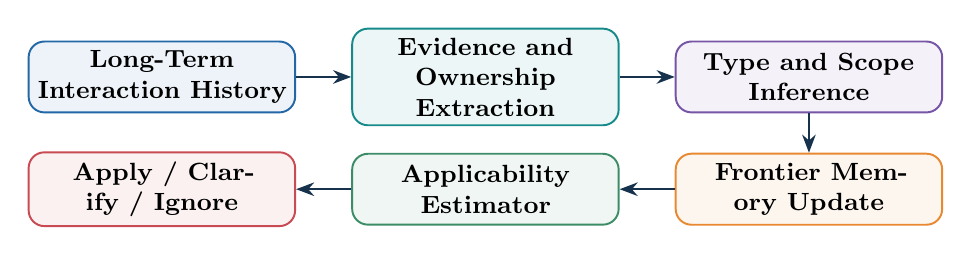
\begin{tikzpicture}[
  node distance=5mm and 7mm,
  box/.style={rounded corners=2mm,minimum height=9mm,text width=3.15cm,align=center,draw=#1,fill=#1!8,line width=.7pt,font=\small\bfseries},
  arr/.style={-{Stealth[length=2.3mm]},line width=.8pt,color=navy}
]
\node[box=blue] (hist) {Long-Term Interaction History};
\node[box=teal,right=of hist] (extract) {Evidence and Ownership Extraction};
\node[box=purple,right=of extract] (type) {Type and Scope Inference};
\node[box=orange,below=of type] (mem) {Frontier Memory Update};
\node[box=green,left=of mem] (est) {Applicability Estimator};
\node[box=red,left=of est] (act) {Apply / Clarify / Ignore};
\draw[arr] (hist) -- (extract);
\draw[arr] (extract) -- (type);
\draw[arr] (type) -- (mem);
\draw[arr] (mem) -- (est);
\draw[arr] (est) -- (act);
\end{tikzpicture}
\end{center}

\textbf{Stage 1 - Structured extraction.} From each conversation chunk, the model extracts candidate claims, owner, speech act (factual, hypothetical, quoted, or role-played), time, local context, and confidence.

\textbf{Stage 2 - Boundary formation and update.} New evidence triggers one of \textsc{Add}, \textsc{Update}, \textsc{Merge}, \textsc{Retract}, \textsc{Expire}, or \textsc{Ignore}. The model distinguishes stable preference from temporary state, current goal, and external constraint.

\textbf{Stage 3 - Context-conditioned applicability.} Given the current query, a lightweight model estimates whether each relevant preference applies. Retrieval is query-conditioned and returns only the preference rule and minimal support evidence.

\textbf{Stage 4 - Active boundary policy.} The model applies a preference when confidence is high, ignores it when the context is outside its scope, and asks one minimal clarification question when the decision lies near the boundary.

\subsection{3.3 Training Strategy}
\begin{enumerate}
  \item \textbf{Structured SFT:} train extraction, information-type classification, boundary construction, ownership, and temporal validity.
  \item \textbf{Counterfactual contrastive training:} use twin histories with similar surface behavior but different latent reasons or scopes; penalize identical downstream behavior when the counterfactual change should matter.
  \item \textbf{Action-policy training:} supervise the \textsc{Apply}/\textsc{Clarify}/\textsc{Ignore} decision and the minimal clarification question.
  \item \textbf{Optional lightweight GRPO:} optimize final answer quality, scope compliance, calibration, and clarification cost after the supervised system is stable.
\end{enumerate}

A compact objective is sufficient:
\[
\mathcal{L}=\mathcal{L}_{\mathrm{memory}}+\lambda_1\mathcal{L}_{\mathrm{scope}}+
\lambda_2\mathcal{L}_{\mathrm{counterfactual}}+\lambda_3\mathcal{L}_{\mathrm{action}}+
\lambda_4\mathcal{L}_{\mathrm{calibration}}.
\]

\section{4. Evaluation Design and Feasibility}

\subsection{4.1 FrontierSuite: a Focused Diagnostic Suite}
The project does \textbf{not} require a new large-scale general benchmark. Instead, it builds a focused diagnostic suite of approximately 600--1,000 contrastive groups derived from or aligned with PersonaMem-v2 and RealPref. Each group contains:

\begin{center}
\begin{tabularx}{0.94\textwidth}{P{3.5cm}Y}
\toprule
\rowcolor{teal!10}
\textbf{Component} & \textbf{Purpose}\\
\midrule
Counterfactual twin histories & Same surface action, different reason or scope.\\
Inside-boundary query & The preference should clearly influence the response.\\
Outside-boundary query & The preference should be ignored.\\
Near-boundary query & The model should ask a targeted clarification question.\\
Structured annotations & Type, owner, scope, temporal validity, evidence, and correct action.\\
\bottomrule
\end{tabularx}
\end{center}

Four bounded domains are sufficient for the first paper: \textbf{writing style, education/explanation, travel, and food/recommendation}. They provide clear context shifts, temporary constraints, role changes, and measurable trade-offs.

\subsection{4.2 Primary Metrics}
\begin{tabularx}{\textwidth}{P{3.25cm}Y}
\toprule
\rowcolor{orange!11}
\textbf{Dimension} & \textbf{Metrics}\\
\midrule
Boundary quality & Scope F1, temporal-validity accuracy, type accuracy, ownership accuracy, evidence attribution.\\
Decision quality & Apply/Clarify/Ignore accuracy, unnecessary clarification rate, near-boundary calibration.\\
Personalization & Inside-boundary accuracy, outside-boundary non-use accuracy, open-ended alignment.\\
Counterfactual behavior & Twin discrimination, counterfactual consistency, overgeneralization rate, personalization regret.\\
Efficiency & Memory size, input tokens, update cost, latency.\\
\bottomrule
\end{tabularx}

\subsection{4.3 Baselines and Ablations}
\textbf{Baselines:} no personalization, full long context, raw-history RAG, fact-based memory, PersonaMem-v2 agentic memory, PersonaTree-style structured memory, RPEval/RP-Reasoner-style selective use, and PersonaDual-style binary mode selection.

\textbf{Ablations:} remove scope, counterfactual training, clarification, confidence, ownership, temporal validity, or information-type separation. These ablations create a clean causal story about which component addresses which failure mode.

\subsection{4.4 Practical Scope}
A credible first implementation is feasible with one 3B--8B open model, structured generation, supervised fine-tuning, and a rule-based or small learned applicability head. GRPO, graph storage, and large-scale human studies are optional enhancements rather than prerequisites. A realistic staged plan is:

\begin{center}
\begin{tabularx}{0.95\textwidth}{P{2.1cm}Y P{2.0cm}}
\toprule
\rowcolor{purple!9}
\textbf{Phase} & \textbf{Deliverable} & \textbf{Risk}\\
\midrule
1. Diagnosis & 150--250 controlled failures on frontier LLMs. & Low\\
2. FrontierSuite & 600--1,000 validated contrastive groups. & Medium\\
3. FrontierMem & Prompted and SFT-trained structured memory. & Medium\\
4. Policy & Apply/Clarify/Ignore controller and final generation. & Medium\\
5. Optional & Lightweight GRPO and human preference study. & Optional\\
\bottomrule
\end{tabularx}
\end{center}

\section{5. Prior Work and Precise Differentiation}

\small
\begin{longtable}{P{2.15cm}P{3.05cm}P{10.65cm}}
\toprule
\rowcolor{navy!10}
\textbf{Work} & \textbf{Primary Contribution} & \textbf{Difference from FrontierMem}\\
\midrule
\endfirsthead
\toprule
\rowcolor{navy!10}
\textbf{Work} & \textbf{Primary Contribution} & \textbf{Difference from FrontierMem}\\
\midrule
\endhead
\midrule
\multicolumn{3}{r}{\scriptsize\color{gray}{Continued on next page}}\\
\endfoot
\bottomrule
\endlastfoot
PersonaMem \cite{personamem} & Dynamic user profiling and cross-scenario personalized response evaluation. & Tests whether preferences are remembered and updated, but does not explicitly model preference-specific applicability conditions or boundary-aware actions.\\
PersonaMem-v2 \cite{personamemv2} & Implicit personas, reinforcement fine-tuning, and a compact agentic text memory. & Compresses user understanding into one free-form memory; FrontierMem stores explicit positive/negative scope, evidence, uncertainty, and a three-way use decision.\\
RealPref \cite{realpref} & Realistic long-horizon preference following with explicit-to-implicit expressions. & Evaluates preference following and unseen scenarios, but not counterfactual causes or inside/outside/near-boundary applicability.\\
NextQuill \cite{nextquill} & Causal effect of user history on model and ground-truth tokens for alignment. & Estimates preference-bearing token effects; FrontierMem asks whether a specific preference is valid in the current context and uses counterfactual histories to test scope rather than token attribution.\\
PREFDISCO \cite{prefdisco} & Proactive preference elicitation in cold-start, just-in-time personalization. & Learns what to ask when preferences are initially unknown; FrontierMem clarifies only near a boundary inferred from long-term memory and evaluates whether stored preferences should transfer.\\
RPEval / RP-Reasoner \cite{rpeval} & Rational, selective use of relevant versus irrelevant personalized memory. & Selects useful memories pragmatically, but does not learn explicit applicability rules, their temporal validity, or counterfactual boundaries from the history.\\
Chameleon \cite{chameleon} & Empirical separation of context-sensitive state from stable trait. & Establishes that state dominates trait in psychological profiles; FrontierMem operationalizes this distinction as updateable memory types and response-use boundaries.\\
PAHF \cite{pahf} & Continual personalization using memory, pre-action clarification, and post-action feedback. & Focuses on online agent adaptation in shopping/manipulation; FrontierMem targets general language personalization and formalizes when a stored preference applies or should be ignored.\\
PUMA \cite{puma} & Latent user-state modeling and action selection under partial observability. & Models future user-state dynamics in counseling; FrontierMem models interpretable preference-level scope and evidence without requiring a full world model.\\
PersonaDual \cite{personadual} & Adaptive switching between objective and personalized reasoning modes. & Makes a broad binary mode choice; FrontierMem makes preference-specific decisions, includes a clarification action, and grounds the decision in long-term boundary memory.\\
PersonaTree \cite{personatree} & Hierarchical lifecycle memory linking evidence, patterns, and persona claims with confidence. & Closest structural-memory work, but it does not encode explicit applies-if/not-if boundaries, counterfactual twin evaluation, or a learned clarification policy.\\
TSM / STALE \cite{tsm,stale} & Temporal event validity, durative memory, and invalidation of stale beliefs. & Address when memories are temporally valid; FrontierMem additionally models task-, role-, goal-, audience-, and constraint-conditioned applicability.\\
CIMemories \cite{cimemories} & Contextual integrity: whether personal attributes should be revealed in different tasks. & Focuses on privacy-sensitive information flow; FrontierMem generalizes contextual scope to ordinary preferences and uses it for personalization, non-use, and clarification.\\
\end{longtable}
\normalsize

\section{6. Novelty Assessment}

\begin{keybox}[What is already known]{orange}
The field already contains dynamic preference benchmarks, implicit persona inference, structured and temporal memory, selective memory utilization, state-trait modeling, active clarification, user-state control, contextual privacy, and causal preference alignment. Therefore, a paper that simply combines ``structured memory + uncertainty + clarification'' would not be sufficiently distinctive.
\end{keybox}

\begin{keybox}[The defensible novelty claim]{green}
Based on the targeted literature reviewed above, the new scientific object is the \textbf{preference applicability boundary}: an interpretable, evidence-grounded rule specifying when an individual preference should and should not affect a response. The proposed work is further differentiated by the joint use of \textbf{counterfactual twin histories}, \textbf{inside/outside/near-boundary evaluation}, and a unified \textbf{Apply/Clarify/Ignore} policy.
\end{keybox}

The novelty claim should be stated cautiously:

\begin{quote}
\emph{To the best of our knowledge, FrontierMem is the first framework to learn explicit applicability boundaries for individual user preferences from long-term interaction and to evaluate them through counterfactual twin histories requiring preference application, non-application, or active clarification.}
\end{quote}

This is stronger and safer than claiming the first causal, contextual, structured, or interactive personalization system, because prior work exists in each of those categories.

\subsection{Why the Project Is Well Defined}
\begin{itemize}
  \item \textbf{Single failure mode:} preference overgeneralization.
  \item \textbf{Single learned object:} the applicability boundary of each preference.
  \item \textbf{Single decision interface:} \textsc{Apply}, \textsc{Clarify}, or \textsc{Ignore}.
  \item \textbf{Controlled evaluation:} counterfactual twins plus three boundary regimes.
  \item \textbf{Measurable success:} scope, calibration, counterfactual discrimination, and downstream response quality.
  \item \textbf{Manageable engineering:} structured SFT is sufficient for the minimum viable paper; RL is optional.
\end{itemize}

\subsection{Main Risks and Mitigations}
\begin{tabularx}{\textwidth}{P{3.4cm}Y}
\toprule
\rowcolor{red!8}
\textbf{Risk} & \textbf{Mitigation}\\
\midrule
``Causal'' overclaim & Use \emph{counterfactual applicability} in the title unless a formal SCM and justified interventions are implemented.\\
Overlap with PersonaTree/RPEval/PersonaDual & Make explicit boundaries, twin histories, and the clarification region the core contributions and primary ablations.\\
Synthetic artifacts & Use paired generation, adversarial filtering, human validation on a representative subset, and cross-dataset testing.\\
Too many memory fields & Keep only type, owner, positive/negative scope, time, evidence, confidence, and permission.\\
Clarification becomes annoying & Optimize unnecessary-question rate and require material expected benefit before asking.\\
Insufficient method novelty & Add contrastive boundary training and calibrated action selection, not only prompting or JSON formatting.\\
\bottomrule
\end{tabularx}

\section{7. Final Positioning}

\begin{summarybox}[Recommended Paper Positioning]
\textbf{Title:} \emph{Beyond ``The User Likes X'': Learning Counterfactual Preference Applicability Boundaries for Personalized LLMs}

\textbf{Method:} FrontierMem

\textbf{Evaluation suite:} FrontierSuite

\textbf{Core contribution:} transform the user profile from a set of unconditional facts into a set of context-conditioned rules that determine whether each preference should be applied, ignored, or clarified.

\textbf{Recommended venues:} ACL/EMNLP are the strongest natural fit. ICLR/NeurIPS become realistic if the counterfactual learning objective, calibration method, and generalization analysis are technically strong rather than purely prompt-engineered.
\end{summarybox}

\begin{center}
\vspace{1mm}
\colorbox{navy}{\parbox{0.94\textwidth}{\centering\color{white}\large\bfseries
True personalization is not knowing what a user prefers; it is knowing when that preference should - and should not - shape the response.}}
\end{center}

\section*{References}
\small
\begin{thebibliography}{99}

\bibitem{personamem}
B. Jiang et al. \emph{Know Me, Respond to Me: Benchmarking LLMs for Dynamic User Profiling and Personalized Responses at Scale}. COLM, 2025. \href{https://arxiv.org/abs/2504.14225}{arXiv:2504.14225}.

\bibitem{personamemv2}
B. Jiang et al. \emph{PersonaMem-v2: Towards Personalized Intelligence via Learning Implicit User Personas and Agentic Memory}. 2025. \href{https://arxiv.org/abs/2512.06688}{arXiv:2512.06688}.

\bibitem{realpref}
Q. Guo, Y. Li, Y. Liu, and B. Hooi. \emph{Towards Realistic Personalization: Evaluating Long-Horizon Preference Following in Personalized User-LLM Interactions}. 2026. \href{https://arxiv.org/abs/2603.04191}{arXiv:2603.04191}.

\bibitem{nextquill}
X. Zhao et al. \emph{NextQuill: Causal Preference Modeling for Enhancing LLM Personalization}. ICLR, 2026. \href{https://arxiv.org/abs/2506.02368}{arXiv:2506.02368}.

\bibitem{prefdisco}
S. S. Li et al. \emph{Personalized Reasoning: Just-In-Time Personalization and Why LLMs Fail at It}. 2025/2026. \href{https://arxiv.org/abs/2510.00177}{arXiv:2510.00177}.

\bibitem{rpeval}
X. Feng, W. Gan, X. Chen, Q. Dai, and Y. Liu. \emph{How Does Personalized Memory Shape LLM Behavior? Benchmarking Rational Preference Utilization in Personalized Assistants}. 2026. \href{https://arxiv.org/abs/2601.16621}{arXiv:2601.16621}.

\bibitem{chameleon}
T. Harry et al. \emph{Beyond Fixed Psychological Personas: State Beats Trait, but Language Models are State-Blind}. 2026. \href{https://arxiv.org/abs/2601.15395}{arXiv:2601.15395}.

\bibitem{pahf}
K. Liang et al. \emph{Learning Personalized Agents from Human Feedback}. 2026. \href{https://arxiv.org/abs/2602.16173}{arXiv:2602.16173}.

\bibitem{puma}
J. Luo et al. \emph{Know You Before You Speak: User-State Modeling for LLM Personalization in Multi-Turn Conversation}. 2026. \href{https://arxiv.org/abs/2605.24647}{arXiv:2605.24647}.

\bibitem{personadual}
X. Liu et al. \emph{PersonaDual: Balancing Personalization and Objectivity via Adaptive Reasoning}. 2026. \href{https://arxiv.org/abs/2601.08679}{arXiv:2601.08679}.

\bibitem{personatree}
Y. Hou et al. \emph{PersonaTree: Structured Lifecycle Memory for Person Understanding in LLM Agents}. 2026. \href{https://arxiv.org/abs/2606.04780}{arXiv:2606.04780}.

\bibitem{tsm}
M. Su et al. \emph{Beyond Dialogue Time: Temporal Semantic Memory for Personalized LLM Agents}. 2026. \href{https://arxiv.org/abs/2601.07468}{arXiv:2601.07468}.

\bibitem{stale}
H. Chao et al. \emph{STALE: Can LLM Agents Know When Their Memories Are No Longer Valid?} 2026. \href{https://arxiv.org/abs/2605.06527}{arXiv:2605.06527}.

\bibitem{cimemories}
N. Mireshghallah et al. \emph{CIMemories: A Compositional Benchmark for Contextual Integrity of Persistent Memory in LLMs}. ICLR, 2026. \href{https://arxiv.org/abs/2511.14937}{arXiv:2511.14937}.

\end{thebibliography}

\end{document}
